\documentclass[a4paper,11pt]{article}

\usepackage[margin=2.3cm]{geometry}
\usepackage{fontspec}
\setmainfont{TeX Gyre Pagella}
\usepackage{unicode-math}
\setmathfont{TeX Gyre Pagella Math}

\usepackage{tikz}
\usetikzlibrary{arrows.meta,calc,positioning,shapes.geometric,decorations.pathmorphing,patterns}

\usepackage{microtype}
\usepackage{enumitem}
\setlist{nosep,leftmargin=*}

\pagestyle{empty}
\setlength{\parindent}{0pt}
\setlength{\parskip}{0.3em}

% Konsistente stilar for alle diagram
\tikzset{
  node-d/.style={draw,fill=black,regular polygon,regular polygon sides=6,minimum size=7mm,inner sep=0pt,text=white,font=\small\itshape},
  node-a/.style={draw,fill=black!70,regular polygon,regular polygon sides=3,minimum size=7mm,inner sep=0pt,text=white,font=\small\itshape},
  node-t/.style={draw,circle,minimum size=7mm,inner sep=0pt,line width=0.8pt,font=\small\itshape},
  node-o/.style={draw,fill=black!15,rectangle,minimum size=7mm,inner sep=0pt,font=\small\itshape},
  node-i/.style={draw,diamond,minimum size=8mm,inner sep=0pt,line width=0.4pt,font=\small\itshape},
  % Komponent-nodar i KK
  comp/.style={draw,rectangle,minimum width=28mm,minimum height=10mm,line width=0.5pt,font=\small,align=center},
  compsmall/.style={draw,rectangle,minimum width=20mm,minimum height=8mm,line width=0.5pt,font=\footnotesize,align=center},
  % Kantar
  impl/.style={-{Latex[length=2mm]},line width=0.5pt},
  exemp/.style={-{Latex[length=2mm]},line width=0.5pt,dashed},
  equiv/.style={{Latex[length=2mm]}-{Latex[length=2mm]},line width=0.7pt,double,double distance=1.2pt},
  post/.style={-{Latex[length=2mm]},line width=0.5pt,dotted},
}

\begin{document}

%===============================================================
%  SIDE 1 — NOTASJONSNØKKEL
%===============================================================
\begin{center}
{\large\scshape Notasjon}\\[0.5em]
{\itshape Ei grafisk grammatikk for Formlære}
\end{center}

\vspace{0.4em}

Notasjonen er rigid. Same symbol tyder same sak i alle figurar. Eit diagram skal lesast utan traktaten i hand.

\vspace{0.3em}

\hrule

\vspace{0.4em}

{\scshape\small Nodar — proposisjonstypar}\\[0.3em]


\begin{tikzpicture}[baseline=(current bounding box.center)]
  \node[node-d] (d) at (0,0) {d};
  \node[node-a] (a) at (3.3,0) {a};
  \node[node-t] (t) at (6.6,0) {t};
  \node[node-o] (o) at (9.9,0) {o};
  \node[node-i] (i) at (13.2,0) {i};
\end{tikzpicture}

\begin{tabular}{@{}p{2.6cm}p{2.6cm}p{2.6cm}p{2.6cm}p{2.6cm}@{}}
\footnotesize definisjon & \footnotesize postulat & \footnotesize teorem & \footnotesize observasjon & \footnotesize illustrasjon\\
\footnotesize\itshape grunnfjell & \footnotesize\itshape peikar & \footnotesize\itshape slutning & \footnotesize\itshape empiri & \footnotesize\itshape døme
\end{tabular}

\vspace{0.4em}

Forma ber typen. Fylt sekskant er ei definisjon; triangel peikar inn eit postulat; open sirkel er ein avslutta slutning; fylt kvadrat er ei flat observasjon; open rombe er eit døme som vendar det abstrakte.

\vspace{0.4em}

\hrule

\vspace{0.4em}

{\scshape\small Kantar — relasjonar}\\[0.6em]

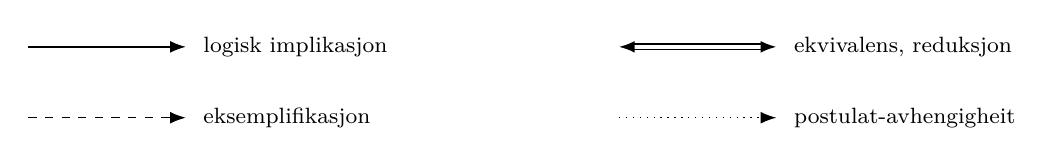
\begin{tikzpicture}[baseline=(current bounding box.center)]
  \draw[impl] (0,0) -- (2,0);      \node[right,font=\footnotesize] at (2.1,0) {logisk implikasjon};
  \draw[exemp] (0,-0.9) -- (2,-0.9);\node[right,font=\footnotesize] at (2.1,-0.9) {eksemplifikasjon};
  \draw[equiv] (7.5,0) -- (9.5,0);  \node[right,font=\footnotesize] at (9.6,0) {ekvivalens, reduksjon};
  \draw[post] (7.5,-0.9) -- (9.5,-0.9);\node[right,font=\footnotesize] at (9.6,-0.9) {postulat-avhengigheit};
\end{tikzpicture}

\vspace{0.4em}

Retninga av pila les frå premiss til slutning. Dobbel pil markerer at to uttrykk er same sak under kvar si kollaps. Prikka pil signaliserer at slutninga kviler på eit postulat, ikkje berre på føregåande proposisjonar.

\vspace{0.4em}

\hrule

\vspace{0.4em}

{\scshape\small Komponentsymbol}\\[0.4em]

\begin{tabular}{@{}lp{14cm}@{}}
$\mathbb{M}$ & formrom, mengda av moglege konfigurasjonar (1.3)\\
$\Pi$ & epistemisk partisjon over $\mathbb{M}$, $(K,\,C,\,F)$ (1.44)\\
$SG$ & formgrammatikk, trippelet $(S,R,\omega)$ (5.3)\\
$\mathcal{L}$ & tilpassingslandskap, vektorsum av seleksjonstrykk (3.1)\\
$\mathcal{A}$ & agenthierarki, mengda av formgjevarar $\{A_0,\dots,A_n\}$ (5.11, 6.12)\\
$A=(m,\pi,\varepsilon)$ & agent: generativ modell, politikk, KL-toleranseterskel (5.11)\\
$C(A)$ & kognitiv lyskjegle / kapasitet: aksar der agenten held $D_{\mathrm{KL}}\le\varepsilon$ (5.2, 5.601)\\
$\omega(A)$ & omhug: vektor $\{D_{\mathrm{KL}}(X_i\mid\pi_A)\}$ over kapasiteten (5.6)\\
\end{tabular}

\vspace{0.4em}

\hrule

\vspace{0.4em}

{\scshape\small Regionar i formrommet}\\[0.6em]

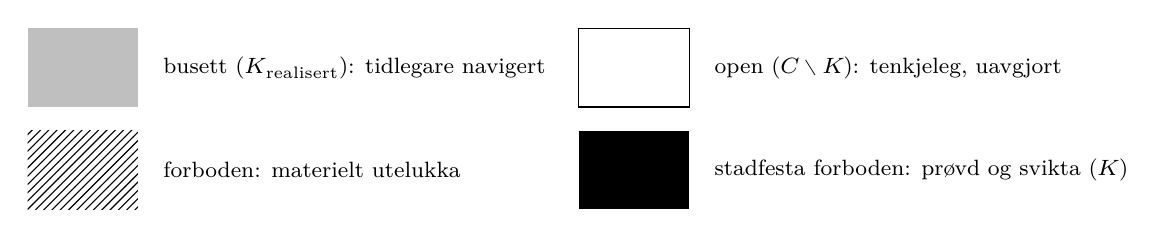
\begin{tikzpicture}[baseline=(current bounding box.center)]
  \fill[black!25] (0,0) rectangle (1.4,1);  \node[right,font=\footnotesize] at (1.6,0.5) {busett ($K_\text{realisert}$): tidlegare navigert};
  \draw (7,0) rectangle (8.4,1);             \node[right,font=\footnotesize] at (8.6,0.5) {open ($C\setminus K$): tenkjeleg, uavgjort};
  \fill[pattern=north east lines] (0,-1.3) rectangle (1.4,-0.3); \node[right,font=\footnotesize] at (1.6,-0.8) {forboden: materielt utelukka};
  \fill[black] (7,-1.3) rectangle (8.4,-0.3); \node[right,font=\footnotesize] at (8.6,-0.8) {stadfesta forboden: prøvd og svikta ($K$)};
\end{tikzpicture}

\vspace{0.4em}

Dei to øvre er opne; dei to nedre er lukka. Skrå strekar markerer det som ikkje er prøvd fordi det ikkje kan prøvast; solid svart markerer det som er prøvd og ikkje verka.

\vspace{0.4em}

\hrule

\vspace{0.4em}

{\scshape\small Operatorar og tidsparametrar}\\[0.4em]

\begin{tabular}{@{}ll@{\hspace{1.2em}}ll@{}}
$\nabla$ & gradient i landskapet &
$\cap$ & skjering mellom lyskjegler\\
$\tau$ & transformasjon i grammatikk &
$\omega$ & starttilstand, grammatikkens null\\
$\rightarrow$ & regelapplikasjon &
$\leftrightarrow$ & gjensidig deformasjon\\
$\uparrow\downarrow$ & emergens, regulering mellom skalaer &
$\varepsilon$ & KL-toleranseterskel (5.11, 5.212)\\
$\tau(A)$ & agentens prediksjonshorisont (5.112) &
$\tau_{\mathrm{mem}}$ & landskapets minnehalveringstid (3.2, 4.3)\\
$\rho_i$ & sviktlatens $\tau(X_i)/\tau(A)$ (7.14) &
$D_{\mathrm{KL}}$ & Kullback--Leibler-divergens\\
\end{tabular}

\newpage

%===============================================================
%  SIDE 2 — KOMPONENTKART (KK)
%===============================================================
\begin{center}
{\large\scshape Komponentkart}\\[0.5em]
{\itshape Kjerne-likninga, proposisjon 5.7 og 8.1, som figur}
\end{center}

\vspace{0.5em}

\begin{center}
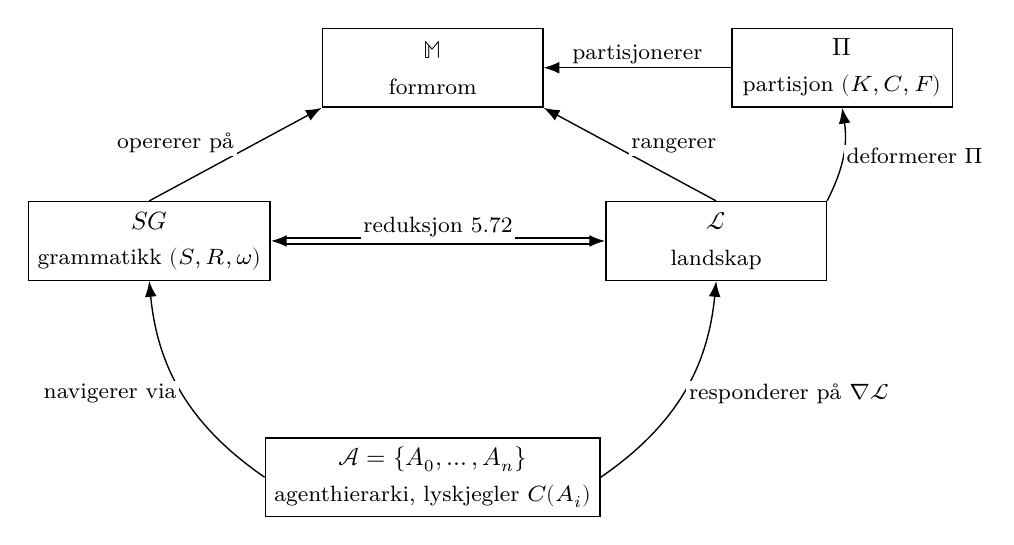
\begin{tikzpicture}[every node/.style={font=\small}]

  % Layout: M i sentrum, dei fire andre rundt. M får inn frå tre sider;
  % agenten står klart nede og sender ut sine tre piler utan kryssing.
  \node[comp] (M)  at (3, 2.2) {$\mathbb{M}$\\[2pt]\footnotesize formrom};
  \node[comp] (P)  at (8.2, 2.2) {$\Pi$\\[2pt]\footnotesize partisjon $(K,C,F)$};
  \node[comp] (SG) at (-0.6, 0) {$SG$\\[2pt]\footnotesize grammatikk $(S,R,\omega)$};
  \node[comp] (L)  at (6.6, 0) {$\mathcal{L}$\\[2pt]\footnotesize landskap};
  \node[comp,minimum width=42mm] (A) at (3, -3.0) {$\mathcal{A}=\{A_0,\dots,A_n\}$\\[2pt]\footnotesize agenthierarki, lyskjegler $C(A_i)$};

  % Kantar mellom komponentane — spesifiserer ankerpunkt for å unngå kryssing
  \draw[impl] (P.west) -- node[above,font=\footnotesize,fill=white,inner sep=1pt] {partisjonerer} (M.east);
  \draw[impl] (SG.north) -- node[above left=-1pt,font=\footnotesize,fill=white,inner sep=1pt] {opererer på} (M.south west);
  \draw[impl] (L.north) -- node[above right=-1pt,font=\footnotesize,fill=white,inner sep=1pt] {rangerer} (M.south east);
  \draw[impl] (L.north east) to[bend right=18] node[right,font=\footnotesize,fill=white,inner sep=1pt] {deformerer $\Pi$} (P.south);
  \draw[impl] (A.west) to[bend left=25] node[left=1pt,font=\footnotesize,fill=white,inner sep=1pt] {navigerer via} (SG.south);
  \draw[impl] (A.east) to[bend right=25] node[right=1pt,font=\footnotesize,fill=white,inner sep=1pt] {responderer på $\nabla\mathcal{L}$} (L.south);
  \draw[equiv] (SG.east) -- node[above,font=\footnotesize,fill=white,inner sep=1pt] {reduksjon 5.72} (L.west);

\end{tikzpicture}
\end{center}

\vspace{0.4em}

\hrule

\vspace{0.4em}

{\scshape\small Lesing}

\vspace{0.3em}

Komponentkartet skal lesast som fem nodar og sju merkte kantar. Ingen komponent står åleine; kvar er definert ved sine inngåande og utgåande relasjonar.

\begin{itemize}
\item $\Pi$ \emph{partisjonerer} $\mathbb{M}$ i busette, opne og forbodne regionar. Partisjonen er epistemisk; ho endrar seg med kvar realisering.
\item $SG$ \emph{opererer på} $\mathbb{M}$ gjennom innleiring. Reglane avgjer kva overgangar som er mogleg.
\item $\mathcal{L}$ \emph{rangerer} $\mathbb{M}$ ved å tilleggje kvar posisjon ein verdi; vektorsum av verksame seleksjonstrykk.
\item $\mathcal{L}$ \emph{deformerer} $\Pi$: nye realiseringar flyttar grensa mellom $K$ og $C$.
\item $\mathcal{A}$ \emph{navigerer via} $SG$ og \emph{responderer på} $\nabla\mathcal{L}$. Agenten oppfinn ikkje målet, han oppdagar gradienten. Kvar $A_i$ ber si eiga lyskjegle $C(A_i)\subseteq\mathbb{M}$; agenten ser berre delar av rommet.
\item Den doble pila mellom $SG$ og $\mathcal{L}$ markerer reduksjonsteoremet 5.72: rein formgrammatikk er kollapsen $\nabla\mathcal{L}\equiv 0$; rein gradientnavigasjon er kollapsen der $SG$ er identitetsoperasjonen på $\mathbb{M}$.
\end{itemize}

\vspace{0.3em}

{\scshape\small Kjerne-likninga i figurform}

\vspace{0.3em}

Den venstre-lesbare kjerne-likninga 5.7,
\[
\text{Form} \;=\; SG\!\left(\nabla_{C(A)}\,\mathcal{L}(c,t)\right),
\]
viser seg i diagrammet som stien $\mathcal{A} \to \mathcal{L} \to \nabla \to SG \to \mathbb{M}$. Den generative forma 8.1,
\[
P(F\mid\{A_i\},\mathcal{L},SG)\;\propto\;\exp\!\left(-\sum_i w_i\,\hat{\mathcal{L}}_i(F)\right),\quad F\in L(SG)\cap\bigcap_i C(A_i),
\]
viser at domenet er skjeringa mellom $SG$ sitt språk og samla lyskjegler, og at vekta er summert over agenthierarkiet.

\end{document}
